\documentclass[a4paper,12pt]{article}
\usepackage{amssymb}
\usepackage{amsmath}
\usepackage{xcolor,color}
\usepackage{tikz}
\usetikzlibrary{shapes.geometric,positioning,decorations.pathreplacing,decorations.pathmorphing,patterns,decorations.markings}

\begin{document}

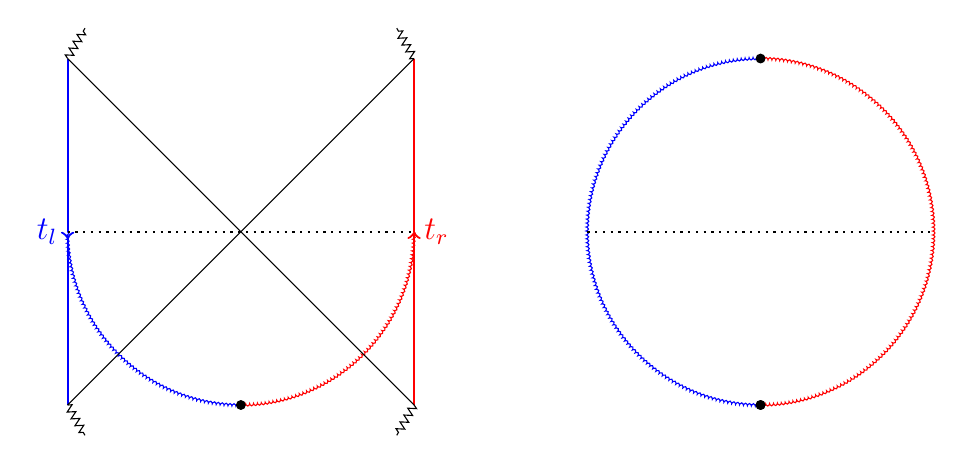
\begin{tikzpicture}[scale=1.1]
\draw[blue, thick,-<](-2,0)--++(0,2);\draw[blue,thick] (-2,2)node[left]{\large$t_l$}--++(0,2);
\draw[thick,red, ->](2,0)--++(0,2);\draw[thick,red] (2,2)node[right]{\large$ t_r$}--++(0,2);
\draw[blue,decoration={coil,segment length=0.5mm,amplitude=0.15mm},decorate] (-2,2) arc (180:270:2);\draw[red,decoration={coil,segment length=0.5mm,amplitude=0.15mm},decorate] (2,2) arc (0:-90:2); \draw[fill=black] (0,0) circle (0.05cm);
 \draw[thick,dotted](-2,2)--++(4,0);
\draw[decoration={zigzag,segment length=1mm,amplitude=0.5mm},decorate](-2,4)--++(0.2,+0.35); 
\draw[decoration={zigzag,segment length=1mm,amplitude=0.5mm},decorate](2,4)--++(-0.2,+0.35); 
\draw[decoration={zigzag,segment length=1mm,amplitude=0.5mm},decorate](-2,0)--++(0.2,-0.35); 
\draw[decoration={zigzag,segment length=1mm,amplitude=0.5mm},decorate](2,0)--++(-0.2,-0.35); 
\draw (-2,0)--++(4,4);
\draw (+2,0)--++(-4,4);
\draw[blue,decoration={coil,segment length=0.5mm,amplitude=0.15mm},decorate] (6,4) arc (90:270:2);\draw[red,decoration={coil,segment length=0.5mm,amplitude=0.15mm},decorate] (6,4) arc (90:-90:2); \draw[fill=black] (6,0) circle (0.05cm);
 \draw[thick,dotted](4,2)--++(4,0);\draw[fill=black] (6,0) circle (0.05cm);
\draw[fill=black] (6,4) circle (0.05cm);
\end{tikzpicture}

\end{document}